
\chapter{Giovedì 28/03/2021 e Venerdì 26/03/2021}
\section{Comandi per la lettura di esami passati}
\small
\begin{multicols}{3}
	\paragraph{Decompressione dei files}
	\begin{verbatim}
		tar xf percorso/nome_file
	\end{verbatim}
	\paragraph{Apertura di un file pdf}
	\begin{verbatim}
		evince percorso/nome_file
	\end{verbatim}
	\paragraph{Lettura di un file} 
	\begin{verbatim}
		cat percorso/nome_file
	\end{verbatim}
\end{multicols}
\normalsize
\section{Esercizio di traduzione [Scritto del 26/02/2020]}
\begingroup
\small
\begin{framed}
	\paragraph{Codice C++ da utilizzare}
	\begin{verbatim}
		struct st1 { char vi[4]; };
		struct st2 { char vd[4]; };
		class cl {
			char v1[4]; int v3[4]; long v2[4];
			public:
			cl(st1& ss);
			cl elab1(char ar1[], st2 s2);   
			
			void stampa() {
				for (int i = 0; i < 4; i++) cout << (int)v1[i] << ’ ’; cout << endl;
				for (int i = 0; i < 4; i++) cout << (int)v2[i] << ’ ’; cout << endl;
				for (int i = 0; i < 4; i++) cout << (int)v3[i] << ’ ’; cout << endl << endl;
			}
		};
	\end{verbatim}
	\paragraph{Codice C++ da tradurre}
	\begin{verbatim}
		cl::cl(st1& ss) {
			for (int i = 0; i < 4; i++) {
				v1[i] = ss.vi[i]; 
				v2[i] = v1[i] / 2;
				v3[i] = 2 * v1[i];
			}
		}
		
		cl cl::elab1(char ar1[], st2 s2) {
			st1 s1;
			for (int i = 0; i < 4; i++) s1.vi[i] = ar1[i] + i;
			
			cl cla(s1);
			for (int i = 0; i < 4; i++) cla.v3[i] = s2.vd[i];
			
			return cla;
		}
	\end{verbatim}
\end{framed}
\paragraph{Traduzione del costruttore}
\begin{verbatim}
	.global _ZN2clC1ER3st1
	_ZN2clC1ER3st1:
	push %rbp
	mov %rsp, %rbp
	sub $32, %rsp
	mov %rdi, -8(%rbp)
	mov %rsi, -16(%rbp)
	
	# inizializzazione
	movl $0, -24(%rbp)
	.Lfor: #confronto
	cmpl $4, -24(%rbp)
	jl .Lcorpo
	jmp .Lfinefor
	.Lcorpo:
	# v1[i] = ss.vi[i]
	movslq -24(%rbp), %rcx
	mov -16(%rbp), %rdi
	mov (%rdi, $rcx), %al
	mov -8(%rbp), %rsi
	mov %al, (%rsi, %rcx)
	
	# v2[i] = v1[i] / 2
	mov (%rsi, %rcx), %al
	sar $1, %al
	movsbq %al, %rax
	mov %rax, 24(%rsi, %rcx, 8)
	
	# v3[i] = 2*v1[i]
	mov (%rsi, %rcx), %al
	shl $1, %al
	movsbl %al, %eax
	mov %eax, 4(%rsi, %rcx, 4)
	
	# incremento     
	inc -24(%rbp)
	jmp .Lfor
	.Lfinefor 
	mov -8(%rbp), %rax
	leave
	ret
\end{verbatim}
\begin{itemize}
	\item Scriviamo il nome della funzione
	\begin{verbatim}
		_ZN2clC1ER3st1
	\end{verbatim}
	consideriamo che si ha una funzione membro, il suo nome, che è un costruttore, che l'unico parametro esplicito presente è un riferimento alla struttura \emph{st1}.
	\item Si consideri la struttura di un qualunque spazio di memoria riservato a un'istanza della classe (considerando, come al solito, \emph{sizeof} e \emph{alignof} dei vari elementi).
	\begin{center}
		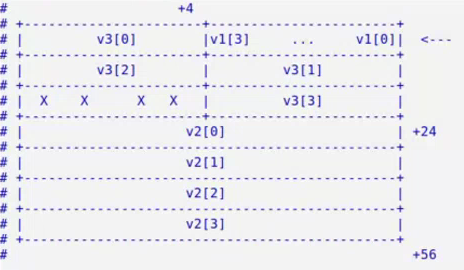
\includegraphics{img/46.PNG}
	\end{center}  
	Si consideri la struttura del record di attivazione
	\begin{center}
		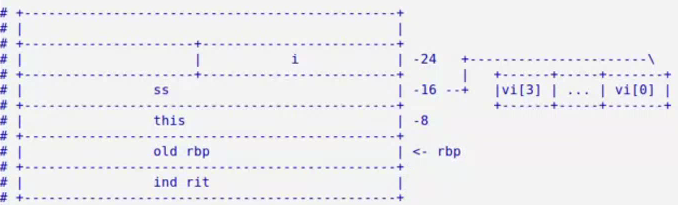
\includegraphics{img/47.PNG}
	\end{center}  
	Presente un puntatore \emph{this} (la funzione che stiamo traducendo è una funzione membro) e un puntatore riguardo il riferimento \emph{ss} (ricordarsi che i riferimenti vengono implementati come puntatori). Seguono i parametri, e dopo le variabili locali (si ricordi che non abbiamo un ordine ben preciso da rispettare, il programma può fare quello che vuole nello spazio che si è riservato nella pila).
	\item Solito prologo
	\begin{verbatim}
		push %rbp
		mov %rsp, %rbp
		sub $32, %rsp
	\end{verbatim}
	inizializziamo anche l'unica variabile locale presente ($i=0$)
	\begin{verbatim}
		movl $0, -24(%rbp)
	\end{verbatim}
	\item Dobbiamo tradurre un \emph{for} in Assembler. Il codice si articola in
	\begin{itemize}
		\item Inizializzazione, eseguita una volta soltanto
		\item Confronto (etichetta .Lfor), La prima jump, condizionata, mi manda al corpo se la condizione è vera. La seconda jump viene raggiunta se la condizione non è vera, e ci permette di saltare a dopo il for (etichetta .Lfinefor).
		\item Corpo del for (etichetta .Lcorpo), che eseguo ogni volta che la condizione risulta vera. All'interno incremento la variabile contatore \emph{i}.
	\end{itemize}
	\item \begin{verbatim}
		v1[i] = ss.vi[i];
	\end{verbatim}
	\begin{itemize}
		\item Attenzione alla variabile contatore \emph{i}: è un intero. Le regole di indirizzamento ci pongono il passaggio a un registro a 64bit. Utilizziamo l'istruzione movslq per estendere con segno l'intero nel passaggio al registro
		\begin{verbatim}
			movslq -24(%rbp), %rcx
		\end{verbatim}
		\item Subito dopo spostiamo l'indirizzo in \emph{ss} in un registro, sempre per questioni di indirizzamento
		\begin{verbatim}
			mov -16(%rbp), %rdi
		\end{verbatim}
		\item A questo punto possiamo spsotare nel registro al (al visto che stiamo lavorando con caratteri)
		\begin{verbatim}
			mov (%rdi, $rcx), %al
		\end{verbatim}
		abbiamo recuperato \emph{ss.vi[i]}.
		\item Abbiamo trovato \emph{ss.vi[i]}, adesso possiamo svolgere l'operazione di assegnamento. Stiamo parlando di un campo della classe. Spostiamo \emph{this} in un registro
		\begin{verbatim}
			mov -8(%rbp), %rsi
		\end{verbatim}
		poniamo, infine, il contenuto del registro al nel vettore da noi detto
		\begin{verbatim}
			mov %al, (%rsi, %rcx)
		\end{verbatim}
	\end{itemize}
	\item \begin{verbatim}v2[i] = v1[i] / 2;\end{verbatim}
	\begin{itemize}
		\item Il valore è quello nel registro al, se ce ne dimentichiamo non è un problema un'istruzione in più
		\begin{verbatim}
			mov (%rsi, %rcx), %al
		\end{verbatim}
		\item La divisione per due si ottiene con uno shift aritmetico a destra
		\begin{verbatim}
			sar $1, %al
		\end{verbatim}
		\item Ci manca l'assegnamento, ma dobbiamo stare attenti alle differenze di tipo: v2 è un array di \emph{long}, v1 un'array di \emph{int}.  Nel passaggio da \emph{int} a \emph{long} dobbiamo fare estensione con segno
		\begin{verbatim}
			movsbq %al, %rax
			mov %rax, 24(%rsi, %rcx, 8)
		\end{verbatim}
		il passaggio da rax è obbligato, non esiste l'istruzione \emph{movsbq} con operando destinatario diverso da registro.
	\end{itemize}
	\item \begin{verbatim}v3[i] = 2 * v1[i];\end{verbatim}
	\begin{itemize}
		\item Recuperiamo \emph{v1[i]}
		\begin{verbatim}
			mov (%rsi, %rcx), %al
		\end{verbatim}
		\item La moltiplicazione per due si ottiene con uno shift logico a sinistra
		\begin{verbatim}
			shl $1, %al
		\end{verbatim} 
		\item Dobbiamo passare da byte a long, con estensione di segno. Si fa in modo simile a come abbiamo gestito il passaggio da byte a quad.
		\begin{verbatim}
			movsbl %al, %eax
			mov %eax, 4(%rsi, %rcx, 4)
		\end{verbatim}
	\end{itemize}
	\item Incremento la variabile \emph{i} memorizzata in memoria
	\begin{verbatim}
		inc -24(%rbp)
	\end{verbatim}
	e ritorno alla condizione
	\begin{verbatim}
		jmp .Lfor
	\end{verbatim}
	\item Concludiamo restituendo l'indirizzo dell'oggetto, e con le solite istruzioni
	\begin{verbatim}
		mov -8(%rbp), %rax <--- restituisco this
		leave
		ret
	\end{verbatim}
\end{itemize}
\paragraph{Traduzione della funzione membro \emph{elab1}} 
\begin{verbatim}
	.global _ZN2cl5elab1EPc3st2
	_ZN2cl5elab1EPc3st2:
	push %rbp
	mov %rsp
	sub $96, %rsp
	mov %rdi, -8(%rbp)
	mov %rsi, -16(%rbp)
	mov %rdx, -24(%rbp)
	mov %ecx, -32%rbp)
	
	# inizializzazione
	movl $0, -28(%rbp)
	.Lfor1: # confronto
	cmpl $4, -28(%rbp)
	jl .Lcorpo1
	jmp .Lfinefor1
	.Lcorpo1:
	movslq -28(%rbp), %rcx
	mov -24(%rbp), %rdi
	movsbl (%rdi, %rcx), %eax
	add %ecx, %eax
	mov %al, -40(%rbp, %rcx)
	
	# inc
	incl -28(%rbp)
	jmp .Lfor1
	.Lfinefor1:
	# &cla -> %rdi   
	lea -96(%rbp), %rdi
	# &s1 -> %rsi
	lea -40(%rbp), %rsi
	
	# secondo for
	# inizializzazione
	movl $0, -28(%rbp)
	1:  # confronto
	cmpl $4, -28(%rbp)
	jl 2f
	jmp 3f
	2:
	# trovo s2.vd[i]
	movslq -28(%rbp), %rcx
	mov -32(%rbp, %rcx), %al
	
	# assegnamento cla.v3[i] = s2.vd[i]
	# attenzione, si assegna un char a un intero ... dobbiamo estendere
	movsbl %al, %eax
	mov %eax, -92(%rbp, %rcx, 4)
	
	# inc
	incl -28(%rbp)
	jmp 1b
	3:
	
	# return cla
	lea -96(%rbp), %rsi
	mov -8(%rbp), %rdi
	mov $7, %rcx
	rep movsq
	
	leave
	ret
\end{verbatim}
\begin{itemize}
	\item Scriviamo il nome della funzione
	\begin{verbatim}
		_ZN2cl5elab1EPc3st2
	\end{verbatim}
	si consideri che \emph{elab1} è una funzione membro, che riceve in ingresso un array di \emph{char} (puntatore al primo elemento) e un oggetto di tipo \emph{st2} passato per valore (ci allarmiamo, ma vediamo che è una struttura banale, di dimensione inferiore a 16 byte, senza costruttori e distruttori, segue un passaggio mediante registri). 
	\item La funzione restituisce un oggetto di tipo \emph{cl} per valore. Purtroppo qua abbiamo un oggetto di dimensione di 56byte: non possiamo passare per registri. Non abbiamo costruttori di copia o distruttori. Il chiamante ci dice dove vuole il risultato (parametro \emph{this}), il chiamato (\emph{elab}) si occupa di inizializzare il risultato (con l'espressione che si trova nel \emph{return}. Non abbiamo un costruttore di copia definito dall'utente, quindi poniamo il costruttore di copia di default (istruzione stringa).
	\begin{framed}
		\item \textbf{Importante}. Attenzione ai parametri impliciti in ingresso. In questo caso dobbiamo inserire sia il puntatore \emph{this} (funzione membro) che il puntatore all'oggetto risultato (poichè l'istanza restituito ha dimensione superiore ai 16byte). Come facciamo?
		\begin{itemize}
			\item In rdi va l'indirizzo dell'oggetto risultato (primo parametro, implicito)
			\item In rsi va \emph{this} (secondo parametro, implicito)
		\end{itemize}
		seguono gli altri parametri.
	\end{framed}
	\item \textbf{Ci sono ottimizzazioni obbligatorie da fare in tutto questo?} No. Potrei utilizzare la NRVO, non allocando \emph{cla} (utilizzo direttamente l'oggetto risultato allocato dal chiamante), ma non è una cosa obbligatoria secondo lo standard \emph{C++ 17}.
	\item In considerazione di tutto quanto vediamo la struttura del record di attivazione:\begin{center}
		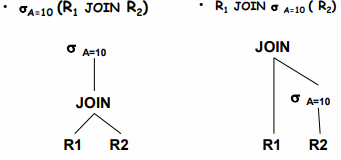
\includegraphics{img/48.PNG}
	\end{center}  
	Ricordarsi che \emph{ar1} è puntatore al primo elemento di un array (lo riscrivo perché sono duro come una pigna). Facciamo il solito prologo
	\begin{verbatim}
		push %rbp
		mov %rsp
		sub $96, %rsp
	\end{verbatim}
	e inizializziamo i vari elementi
	\begin{verbatim}
		mov %rdi, -8(%rbp)
		mov %rsi, -16(%rbp)
		mov %rdx, -24(%rbp)
		mov %ecx, -32%rbp)
	\end{verbatim}
	anche la variabile \emph{i}
	\begin{verbatim}
		movl $0, -28(%rbp)
	\end{verbatim}
	\item Per gestire il for dobbiamo utilizzare delle etichette, come già visto prima. Ricordiamoci che il compilatore vede solo etichette, non ha in testa il concetto di funzione. Segue che le etichette dovranno avere nomi diversi da quelli utilizzati in altre funzioni.
	\item Corpo del primo for:
	\begin{itemize}
		\item Ad ogni iterazione dobbiamo eseguire la seguente operazione
		\begin{verbatim}
			s1.vi[i] = ar1[i] + i;
		\end{verbatim}
		\item Per prima cosa prendiamoci il contenuto del contatore \emph{i}
		\begin{verbatim}
			movslq -28(%rbp), %rcx
		\end{verbatim}
		\item Prendiamo l'indirizzo dell'array \emph{ar1}
		\begin{verbatim}
			mov -24(%rbp), %rdi
		\end{verbatim}
		\item Prendiamo l'elemento dell'array $i-$esimo, estendendolo con segno
		\begin{verbatim}
			movsbl (%rdi, %rcx), %eax
		\end{verbatim}
		\item Aggiungiamo \emph{i} all'elemento \emph{ar1[i]} trovato prima
		\begin{verbatim}
			add %ecx, %eax
		\end{verbatim}
		\item Eseguo l'operazione di assegnamento
		\begin{verbatim}
			mov %al, -40(%rbp, %rcx)
		\end{verbatim}
		\item Concludo alla solita maniera, incremento il contatore \emph{i} e salto alla condizione
		\begin{verbatim}
			incl -28(%rbp)
			jmp .Lfor1
		\end{verbatim}
	\end{itemize}
	\item Necessario chiamare il costruttore di copia per inizializzare l'istanza \emph{cla} di \emph{c1}. Passiamo l'indirizzo dell'oggetto risultato (che contiene i dati dell'istanza)
	\begin{verbatim}
		lea -96(%rbp), %rdi
	\end{verbatim}
	non conosciamo l'indirizzo di \emph{cla}, ma sappiamo come calcolarlo.  L'unico parametro in ingresso esplicito è un riferimento a un'istanza della struttura \emph{st1}.
	\begin{verbatim}
		lea -40(%rbp), %rsi
	\end{verbatim}
	segue la chiamata del costruttore
	\begin{verbatim}
		call _ZN2clC1ER3st1
	\end{verbatim}
	\item Corpo del secondo for
	\begin{itemize}
		\item Inizializziamo nuovamente la variabile contatore, la stessa utilizzata nel primo for
		\begin{verbatim}
			movl $0, -28(%rbp)
		\end{verbatim}
		\begin{framed}
			\item Abbiamo posto le etichette del for in modo diverso rispetto a quello tradizionale. Precisamente:
			\begin{itemize}
				\item Abbiamo posto come "etichette" i numeri \emph{1,2,3}. Etichette tra virgolette perché non rimarranno nel file oggetto: servono soltanto al compilatore per calcolare gli indirizzi verso cui fare jump.
				\item Nelle istruzioni jump abbiamo indicato uno dei tre numeri e una lettera. In particolare
				\begin{itemize}
					\item \begin{verbatim}jl 2f\end{verbatim}indichiamo di voler saltare, con condizione soddisfatta, alla prima "etichetta" 2 che troviamo andando avanti (f per \emph{forward}).
					\item \begin{verbatim}jmp 1b\end{verbatim}indichiamo di voler saltare, in qualunque caso, alla prima "etichetta" 1 che troviamo andando indietro (b per \emph{backward}).
				\end{itemize}
				\item La comodità principale sta nell'indicare, in ogni for, le "etichette" \emph{1,2,3} senza dover inventare, ogni volta, etichette diverse per ogni step del for.
			\end{itemize}
		\end{framed}
		\item Ad ogni iterazione dobbiamo eseguire la seguente operazione
		\begin{verbatim}
			cla.v3[i] = s2.vd[i];
		\end{verbatim}
		\item Poniamo \emph{s2.vd[i]} nel registro al
		\begin{verbatim}
			movslq -28(%rbp), %rcx # Sposto il valore di i in rcx (necessario reg. a 64bit)
			mov -32(%rbp, %rcx), %al
		\end{verbatim}
		\item Eseguiamo l'assegnamento
		\begin{verbatim}
			movsbl %al, %eax
			mov %eax, -92(%rbp, %rcx, 4)
		\end{verbatim}
		si consideri che avviene il passaggio da un char a un intero, quindi dobbiamo fare l'estensione con segno (per fare ciò siamo costretti a scrivere un ulteriore istruzione coinvolgendo il reg. eax)
		\item Concludo alla solita maniera, incremento il contatore \emph{i} e salto alla condizione
		\begin{verbatim}
			incl -28(%rbp)
			jmp 1b
		\end{verbatim}
	\end{itemize}
	\item Andiamo all'istruzione \emph{return}:
	\begin{itemize}
		\item La dimensione dell'oggetto restituito è superiore ai 16byte, quindi non utilizzeremo i registri per passare l'oggetto restituito. Ricordarsi che abbiamo posto nel registro rdi l'indirizzo dell'oggetto risultato. Il chiamante ha allocato lo spazio, noi dobbiamo limitarci ad inizializzarlo.
		\item L'inizializzazione dipende dall'espressione nel return, cioè \emph{cla}. Il costruttore di copia non c'è, quindi si ricorre al costruttore di default (copia membro a membro).
		\item Per copiare tutto \emph{cla} dentro l'oggetto allocato dal chiamante dobbiamo utilizzare le istruzioni stringa
		\begin{verbatim}
			lea -96(%rbp), %rsi
			mov -8(%rbp), %rdi
			mov $7, %rcx
			rep movsq
		\end{verbatim}
		ponendo, come al solito, \emph{source}, \emph{destination} e numero di volte in cui la copia deve essere ripetuta.
	\end{itemize}
	\item Concludiamo come al solito
	\begin{verbatim}
		leave
		ret
	\end{verbatim}
\end{itemize}
\paragraph{Introduzione del costruttore di copia}
Modifichiamo il codice c++ iniziale introducendo un costruttore di copia. La domanda che sorge spontanea è: cosa cambia nelle traduzioni scritte fino ad ora? 
\begin{verbatim}
	struct st1 { char vi[4]; };
	struct st2 { char vd[4]; };
	class cl {
		char v1[4]; int v3[4]; long v2[4];
		public:
		cl(st1& ss);
		cl(const cl& c); # <------------
		...
		...
	\end{verbatim}
	\paragraph{Modifica della \emph{elab1}} Dobbiamo sostituire la parte relativa al costruttore di copia di default limitandoci a chiamare il costruttore di copia da noi definito.
	\begin{verbatim}
		...
		...
		3:
		mov -8(%rbp), %rdi
		lea -96(%rbp), %rsi
		call _ZN2clC1ERKS_
		
		leave
		ret
	\end{verbatim}
	Si osservi che non è necessario porre prima della \emph{leave} il parametro da restituire
	\begin{verbatim}
		mov -8(%rbp), %rax
	\end{verbatim}
	ci pensa il costruttore di copia!
	\paragraph{Proviamo a scrivere il costruttore di copia} Scriviamo il codice Assembler
	\begin{verbatim}
		global _ZN2clC1ERKS_
		_ZN2clC1ERKS_:
		push %rbp
		mov %rsp, %rbp
		mov $rdi, %rdx
		
		mov $7, %rcx
		rep movsq
		mov -8(%rbp), %rax
		
		movb $42, (%rdx)
		leave
		ret
	\end{verbatim}
	\begin{itemize}
		\item Abbiamo scritto un costruttore di copia che non si limita a copiare come il costruttore di copia di default, ma fa anche qualcos'altro. Poniamo per comodità la traduzione in C++ del costruttore appena scritto
		\begin{verbatim}
			cl:cl(const cl&c) {
				for(int i = 0; i < 4; i++) {
					v1[i] = c.v1[i];
					v2[i] = c.v2[i];
					v3[i] = c.v3[i];
				}
				v1[0] = 42; # <----- ecco
			}
		\end{verbatim}
		\item A questo punto ci chiediamo: l'output sarà quello che ci aspettiamo? No, a causa della NRVO. Non viene proprio chiamato il costruttore di copia, poichè non alloco \emph{cla} e utilizzo direttamente lo spazio indicato dal chiamante attraverso l'apposito parametro implicito. 
		\item L'ottimizzazione determina un output diverso. Ponendo nell'istruzione
		\begin{verbatim}
			-fno-elide-constructors
		\end{verbatim}
		diciamo a g++ di non elidere i costruttori. A questo punto l'output dovrebbe essere quello immaginato.
	\end{itemize}
	\endgroup
	
	\section{Esercizio di traduzione [Scritto del 19/09/2018]}
	\begingroup
	\small
	\paragraph{Codice C++ da utilizzare}
	\begin{verbatim}
		struct st1 { char vc[4]; }; struct st2 { int vd[4]; };
		class cl {
			st1 c1; st1 c2; long v[4];
			public:
			cl(char c, st2& s);
			void elab1(st1 s1, st2 s2);
			void stampa() {
				for (int i=0; i < 4; i++) cout << c1.vc[i] << ’ ’; cout << "\n";
				for (int i=0; i < 4; i++) cout << c2.vc[i] << ’ ’; cout << "\n";
				for (int i=0; i < 4; i++) cout << v[i] << ’ ’; cout << "\n\n";
			}
		};
	\end{verbatim}
	\paragraph{Codice C++ da tradurre}
	\begin{verbatim}
		cl::cl(char c, st2& s2) {
			for (int i = 0; i < 4; i++) {
				c1.vc[i] = c; c2.vc[i] = c++;
				v[i] = s2.vd[i] + c2.vc[i];
			}
		}
		cl& cl::elab1(st1 s1, st2 s2) {
			cl cla(’a’, s2);
			for (int i = 0; i < 4; i++) {
				if (c2.vc[i] <= s1.vc[i]) {
					c1.vc[i] = i + cla.c2.vc[i];
					v[i] = i - cla.v[i];    
				}
			}
			return *this;
		}
	\end{verbatim}
	\paragraph{Traduzione della funzione \emph{elab1}}
	\begin{verbatim}
		global _ZN2cl5elab1E3st13st2
		_ZN2cl5elab1E3st13st2:
		push %rbp
		mov %rsp, %rbp
		sub $96, %rsp
		
		mov %rdi, -8(%rbp)
		mov %esi, -16(%rbp)
		mov %rdx, -32(%rbp)
		mov %rcx, -24(%rbp)
		
		# cl cla(`a', s2)     
		lea -80(%rbp), %rdi
		mov $'a', %sil
		lea -32(%rbp), %rdx
		call _ZN2clC1EcR3st2
		
		# init
		movl $0, -40(%rbp)
		.Lfor: # confronto
		cmpl $4, -40(%rbp)
		jl .Lcorpo
		jmp .Lfinefor
		.Lcorpo:
		# test
		mov -8(%rbp), %rdi
		movslq -40(%rbp), %rcx
		mov 4(%rdi, %rcx), %al
		cmpb %al, -16(%rbp, %rcx)
		jle .Lcorpoif
		jmp .Lfineif # se falso salto a fineif
		.Lcorpoif:
		# c1.vc[i] = i + cla.c2.vc[i];
		movsbl -78(%rbp, %rcx), %eax
		add %ecx, %eax
		mov %al, (%rdi, %rcx)
		
		# v[i] = i - cla.v[i];    
		mov -72(%rbp, %rcx, 8), %rax
		sub %rcx, %rax
		mov %rax, 8(%rdi, %rcx, 8)
		.Lfineif:
		# incrmeento
		incl -40(%rbp)
		jmp .Lfor
		.Lfinefor:
		mov -8(%rbp), %rax
		
		leave
		ret
	\end{verbatim}
	
	\begin{itemize}
		\item Consideriamo i parametri in ingresso: abbiamo un'istanza \emph{s1} della struttura \emph{st1}, e un'istanza \emph{s2} della struttura \emph{st2}. Si consideri il parametro implicito \emph{this} posto nel registro \emph{rdi}, visto che \emph{elab1} è una funzione membro della classe \emph{cl}. Si consideri la struttura delle due classi: al loro interno sono presenti, rispettivamente, un array di \emph{char} e un array di \emph{int}.
		\item Scriviamo il nome dell'etichetta della funzione
		\begin{verbatim}
			_ZN2cl5elab1E3st13st2
		\end{verbatim}
		\item La funzione restituisce un riferimento a un oggetto di tipo \emph{cl}, quindi non si ha il solito passaggio per valore. Non dobbiamo costruire un oggetto che la funzione dovrà inizializzare. L'implementazione avviene sottoforma di puntatore, quindi le dimensioni non sono problematiche e l'oggetto viene restituito via registri (non c'è bisogno di un ulteriore parametro implicito).
		\item All'interno abbiamo una variabile locale, precisamente un'istanza \emph{cla} diella classe emph{cl}. Si considerino i dati appartenenti alla classe: due istanze della struttura \emph{st1} e un array di \emph{long}.
		\item In considerazione di quanto detto vediamo la struttura del record di attivazione
		\begin{center}
			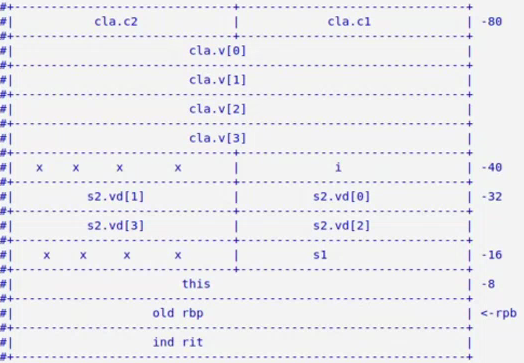
\includegraphics{img/49.PNG}
		\end{center}  
		Abbiamo il puntatore \emph{this} (necessario, \emph{elab1} è una funzione membro), i parametri locali (\emph{s1} ed \emph{s2}), le variabili locali (\emph{cla}). Nell'allineamento degli elementi di \emph{s1} ed \emph{s2} abbiamo un certo margine di movimento, stessa cosa non possiamo dire nell'allineamento degli elementi di \emph{cla} (due istanze di \emph{st1}, ciascuna di 4byte, e un array di 4long, ciascuno di dimensione di 8byte). Scriviamo il solito prologo
		\begin{verbatim}
			push %rbp
			mov %rsp, %rbp
			sub $96, %rsp
		\end{verbatim}
		\item Inizializziamo le variabili locali
		\begin{verbatim}
			mov %rdi, -8(%rbp) # this
			mov %esi, -16(%rbp) # s1
			
			mov %rdx, -32(%rbp) # s2.vd[0], s2.vd[1]
			mov %rcx, -24(%rbp) # s2.vd[3], s2.vd[2]
		\end{verbatim}
		la variabile \emph{i} sarà inizializzata più avanti, quando gestiremo il for. Per quanto riguarda l'istanza \emph{cla} della classe \emph{cl} dobbiamo chiamare l'unico costruttore definito nel codice C++. 
		\begin{verbatim}
			lea -80(%rbp), %rdi
			mov $'a', %sil
			lea -32(%rbp), %rdx
			call _ZN2clC1EcR3st2
		\end{verbatim}
		Prima di chiamare il costruttore abbiamo indicato i parametri in ingresso: con le istruzioni lea abbiamo sistemato il puntatore \emph{this} e il riferimento \emph{s}, con la mov abbiamo indicato il valore della variabile \emph{char}. 
		\item Gestiamo l'unico for presente. A differenza di altri esercizi dobbiamo occuparci anche di un if, presente nel corpo del for.
		\begin{itemize}
			\item Inizializziamo la variabile contatore \emph{i}
			\begin{verbatim}
				movl $0, -40(%rbp)
			\end{verbatim}
			\item Gestiamo l'if introducendo ulteriori etichette. 
			\begin{itemize}
				\item I jump legati al controllo della condizione dell'if vengono posti come nel for, in modo da non dover verificare la condizione opposta (il programma è più intuitivo per chi legge).
				\begin{verbatim}
					mov -8(%rbp), %rdi
					movslq -40(%rbp), %rcx 
					mov 4(%rdi, %rcx), %al 
					cmpb %al, -16(%rbp, %rcx)
					jle .Lcorpoif
					jmp .Lfineif # se falso salto a fineif
				\end{verbatim}
				Utilizziamo le prime due righe per porre in registri il puntatore \emph{this} e la variabile contatore \emph{i} (che va in rdx, a 64bit, per questioni di indirizzamento). Per quanto riguarda il confronto dobbiamo paragonare due cose che stanno in memoria: non possiamo porre due indirizzi di memoria in una stessa istruzione, segue che uno dei due elementi parte del confronto dovrà essere spostato in un registro.
				\item Gestiamo le due operazioni di assegnamento
				\begin{itemize}
					\item 
					\begin{verbatim} 
						# c1.vc[i] = i + cla.c2.vc[i];
						movsbl -78(%rbp, %rcx), %eax
						add %ecx, %eax
						mov %al, (%rdi, %rcx)
					\end{verbatim}
					Per il primo assegnamento: sposto nel registro eax \emph{cla.c2.vc[i]}, sommo ad esso il registro rcx (dove si trova il valore di \emph{i}), pongo il valore sommato in \emph{c1.vc[i]}.
					\item 
					\begin{verbatim}
						# v[i] = i - cla.v[i];    
						mov -72(%rbp, %rcx, 8), %rax
						sub %rcx, %rax
						mov %rax, 8(%rdi, %rcx, 8)
					\end{verbatim}
					Per il secondo assegnamento: sposto nel registro rax \emph{cla.v[i]}, sottraggo a rax il contenuto del registro rcx (dove si trova il valore di \emph{i}), pongo il risultato della sottrazione in \emph{v[i]}.
				\end{itemize}
			\end{itemize}
		\end{itemize}
		\item Per quanto riguarda l'oggetto da restituire consideriamo che dobbiamo ottenere un riferimento. 
		\begin{verbatim}
			return *this;
		\end{verbatim}
		l'operatore di dereferenziazione è necessario per creare un riferimento all'oggetto puntato da \emph{this}. La cosa si traduce in Assembler passando mediante registro l'indirizzo dell'oggetto puntato da \emph{this}.
		\begin{verbatim}
			mov -8(%rbp), %rax
		\end{verbatim}
		\item Concludiamo come al solito con \emph{leave} e \emph{ret}.
	\end{itemize}
	\endgroup